\documentclass[a4paper,12pt]{article}
\usepackage{amsmath,amssymb,amsfonts,amsthm}
\usepackage{tikz}
\usepackage [utf8x] {inputenc}
\usepackage [T2A] {fontenc} 
\usepackage[russian]{babel}
\usepackage{cmap, upgreek}
\usepackage{textcomp} 

% Так ссылки в PDF будут активны
\usepackage[unicode]{hyperref}

% вы сможете вставлять картинки командой \includegraphics[width=0.7\textwidth]{ИМЯ ФАЙЛА}
% получается подключать, как минимум, файлы .pdf, .jpg, .png.
\usepackage{graphicx}
% Если вы хотите явно указать поля:
\usepackage[margin=1in]{geometry}
% Или если вы хотите задать поля менее явно (чем больше DIV, тем больше места под текст):
% \usepackage[DIV=10]{typearea}

\usepackage{fancyhdr}

\newcommand{\bbR}{\mathbb R}%теперь вместо длинной команды \mathbb R (множество вещественных чисел) можно писать короткую запись \bbR. Вместо \bbR вы можете вписать любую строчку букв, которая начинается с '\'.
\newcommand{\eps}{\varepsilon}
\newcommand{\bbN}{\mathbb N}
\newcommand{\dif}{\mathrm{d}}

\newtheorem{Def}{Определение}


\pagestyle{fancy}
\makeatletter % сделать "@" "буквой", а не "спецсимволом" - можно использовать "служебные" команды, содержащие @ в названии
\fancyhead[L]{\footnotesize Электричество и магнетизм}%Это будет написано вверху страницы слева
\fancyhead[R]{\footnotesize ФМХФ МФТИ}
\fancyfoot[L]{\footnotesize \@author}%имя автора будет написано внизу страницы слева
\fancyfoot[R]{\thepage}%номер страницы —- внизу справа
\fancyfoot[C]{}%по центру внизу страницы пусто

\renewcommand{\maketitle}{%
	\noindent{\bfseries\scshape\large\@title\ \mdseries\upshape}\par
	\noindent {\large\itshape\@author}
	\vskip 2ex}
\makeatother
\def\dd#1#2{\frac{\partial#1}{\partial#2}}


\title{3.3.4 \\ Эффект Холла в полупроводниках}
\author{Егор Берсенев} 
\date{15 апреля 2016 г.}

\begin{document}
	\maketitle
	\section{Цель работы}
		 Измерить концентрацию и подвижность носителей заряда в полупроводнике.
	\section{Оборудование}
		Электромагнит с источником питания, миллиамперметр, милливеберметр, реостат, цифровой вольтметр, источник питания, образец легированного германия.
	\section{Теоретическая часть}
		Одновременное исследование эффекта Холла и проводимости позволяет находить плотность носителей заряда и их подвижность. Суть эффекта Холла состоит в следующем. Пусть через однородную пластину металла вдоль оси $x$ течет ток $I$. Если эту пластину поместить в магнитное поле, направленно по оси $y$, то между гранями появится раность потенциалов. На электрон, движущийся со скоростью $\mathbf{b}$ в электромагнитном поле, действует сила Лоренца.
		\begin{equation}
			\mathbf{F_\text{л}} = -e\mathbf{E} - e\mathbf{v} \times \mathbf{B}
		\end{equation}
		В нашем случае сила, обусловленная вторым слагаемым, направлена вдоль оси $z$.
		\begin{equation}
			F_B = e\left|v_x\right|B
		\end{equation}
		Под действием этой силы электроны отклоняются к грани Б, заряжая ее отрицательно. При этом на грани А накапливаются нескомпенсированные положительные заряды, что приводит к возникновению электрического поля $E_z$, направленного от А к Б, которое действует на электроныс силой $F_E = eE_z$, направленной против силы $F_B$.  В стационарном режиме $F_E$ уравновешивает $F_B$, и накопление зарядов на боковых гранях прекращается. Из условия равновесия найдем:
		\begin{equation}
			E_z = \left|v_x\right|B
		\end{equation}
		С полем $E_z$ связана разность потенциалов $U_{\text{АБ}}$ между гранями А и Б.
		\begin{equation}
			U_{\text{АБ}} = - E_zl = - \left|v_x\right|Bl
		\end{equation}
		Заметим, что сила тока
		\begin{equation}
			I = ne\left|v_x\right|l\cdot a,
		\end{equation}
		отсюда найдем ЭДС Холла:
		\begin{equation}
			\upvarepsilon_x = U_{\text{АБ}} = -\frac{IB}{nea} = -R_x\cdot\frac{IB}{a}
		\end{equation}
		\section{Ход работы}
		\subsection{Калибровка электромагнита}
		Проведем калибровку электромагнита:
		\begin{center}
			\begin{tabular}{l|l|l}
				$I$, A    & $\Upphi_0$, мВб   & $\Upphi_1$, мВб   \\ \hline
				0.9  & 6.9  & 1.1 \\
				0.8  & 6.4  & 1.1 \\
				0.7  & 5.9  & 1.1 \\
				0.6  & 5.2  & 1.1 \\
				0.5  & 4.6  & 1.1 \\
				0.4  & 3.9  & 1.1 \\
				0.3  & 3.25 & 1.1 \\
				0.2  & 2.6  & 1.1 \\
				0.15 & 5.2  & 4.2 \\
				0    & 4.35 & 4.2 \\
			\end{tabular}
		\end{center}
		Построим таблицу измерений:
		\begin{center}
			    \begin{tabular}{l|lllllll}
			    	$I$, A    & 0.3    & 0.4    & 0.5   & 0.6    & 0.7    & 0.8    & 0.9    \\
			    	$U_0$, mV & -0.004 & -0.007 & -0.01 & -0.013 & -0.014 & -0.017 & -0.019 \\ \hline
			    	0.1  & 0.005  & 0.008  & 0.007 & 0.007  & 0.008  & 0.09   & 0.01   \\
			    	0.2  & 0.015  & 0.02   & 0.024 & 0.025  & 0.034  & 0.039  & 0.043  \\
			    	0.3  & 0.027  & 0.035  & 0.043 & 0.051  & 0.06   & 0.068  & 0.076  \\
			    	0.4  & 0.038  & 0.05   & 0.062 & 0.075  & 0.088  & 0.098  & 0.111  \\
			    	0.5  & 0.049  & 0.075  & 0.08  & 0.097  & 0.112  & 0.131  & 0.147  \\
			    	0.6  & 0.06   & 0.079  & 0.099 & 0.120  & 0.140  & 0.158  & 0.176  \\
			    	0.7  & 0.07   & 0.093  & 0.115 & 0.120  & 0.163  & 0.184  & 0.210  \\
			    	0.8  & 0.083  & 0.107  & 0.132 & 0.160  & 0.186  & 0.210  & 0.240  \\
			    	0.9  & 0.09   & 0.0119 & 0.147 & 0.179  & 0.207  & 0.237  & 0.265  \\
			    \end{tabular}
		\end{center}
		Построим графики:
		
		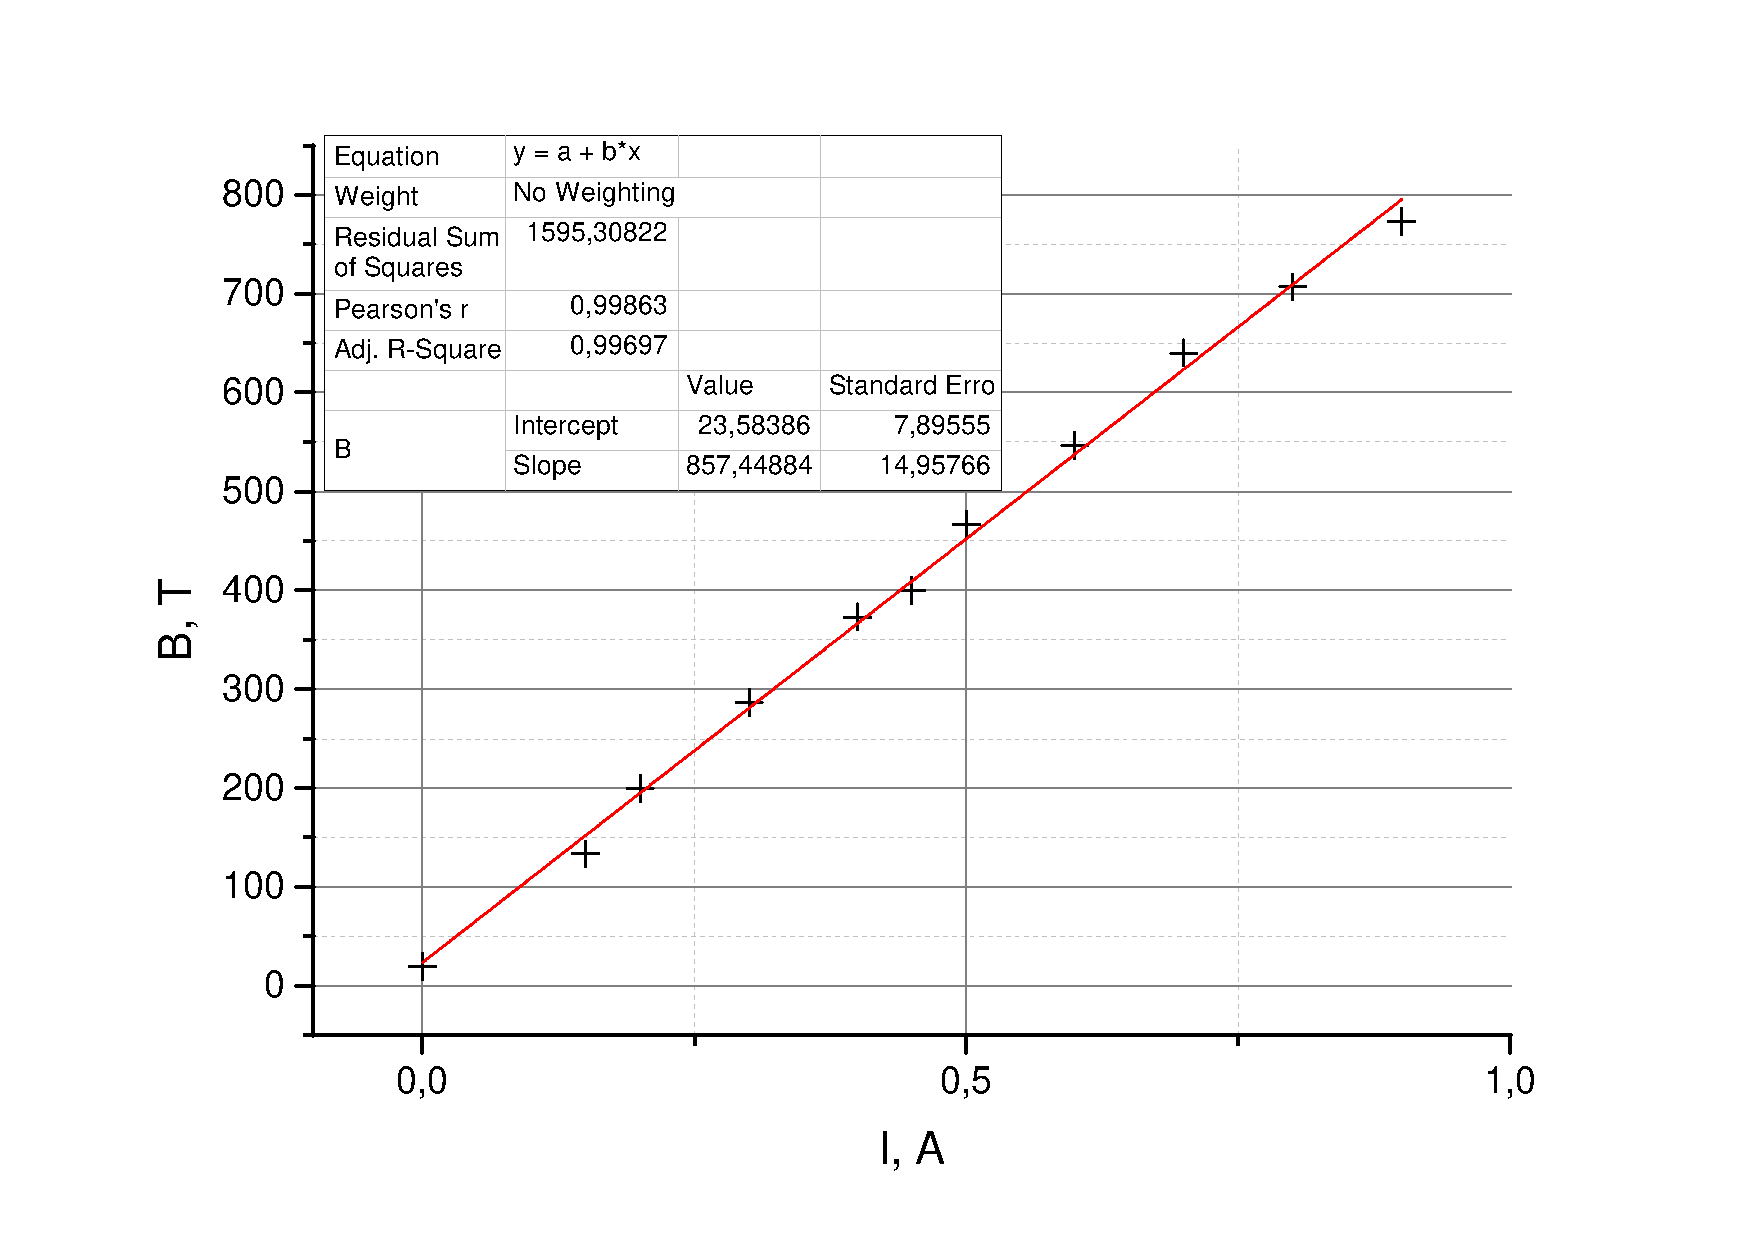
\includegraphics[width = 0.8\linewidth]{BIM}
		
		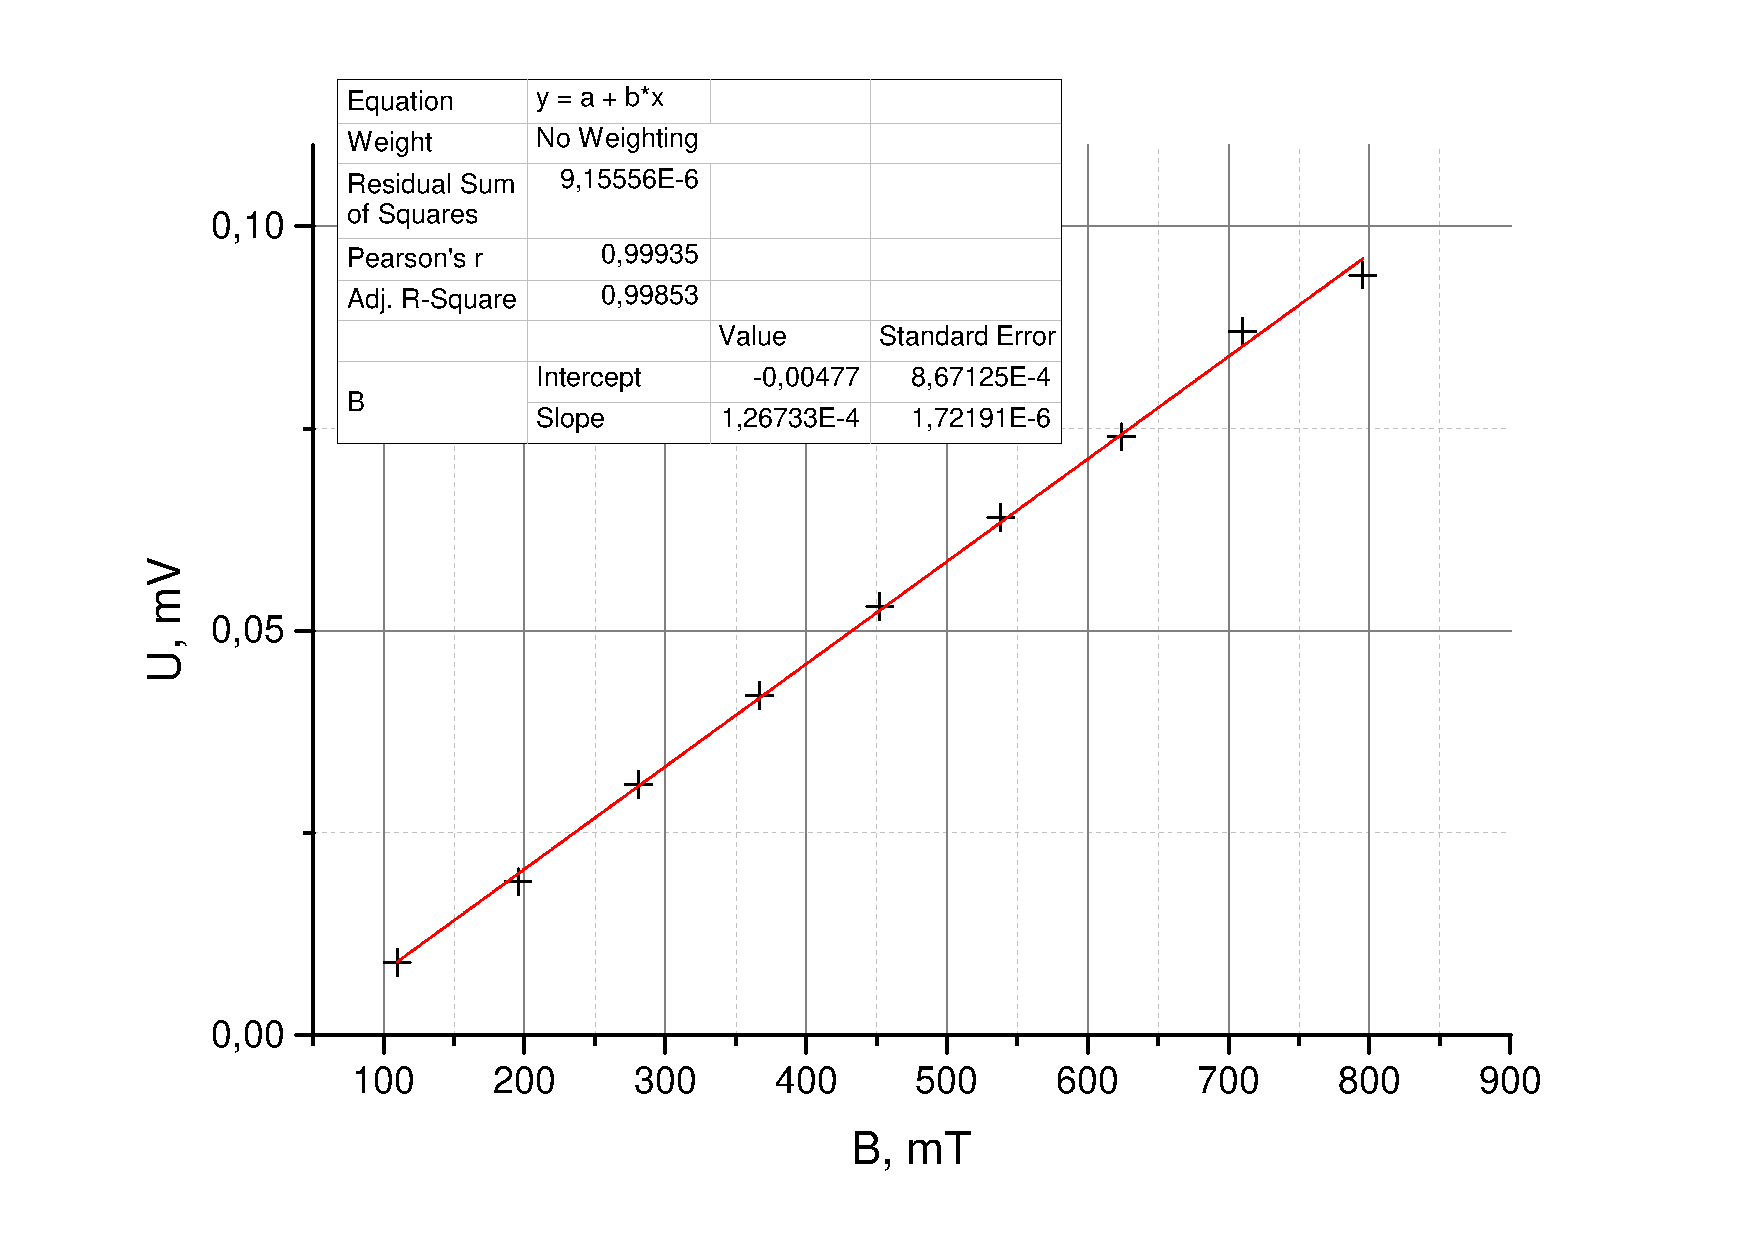
\includegraphics[width = 0.8\linewidth]{A03}
		
		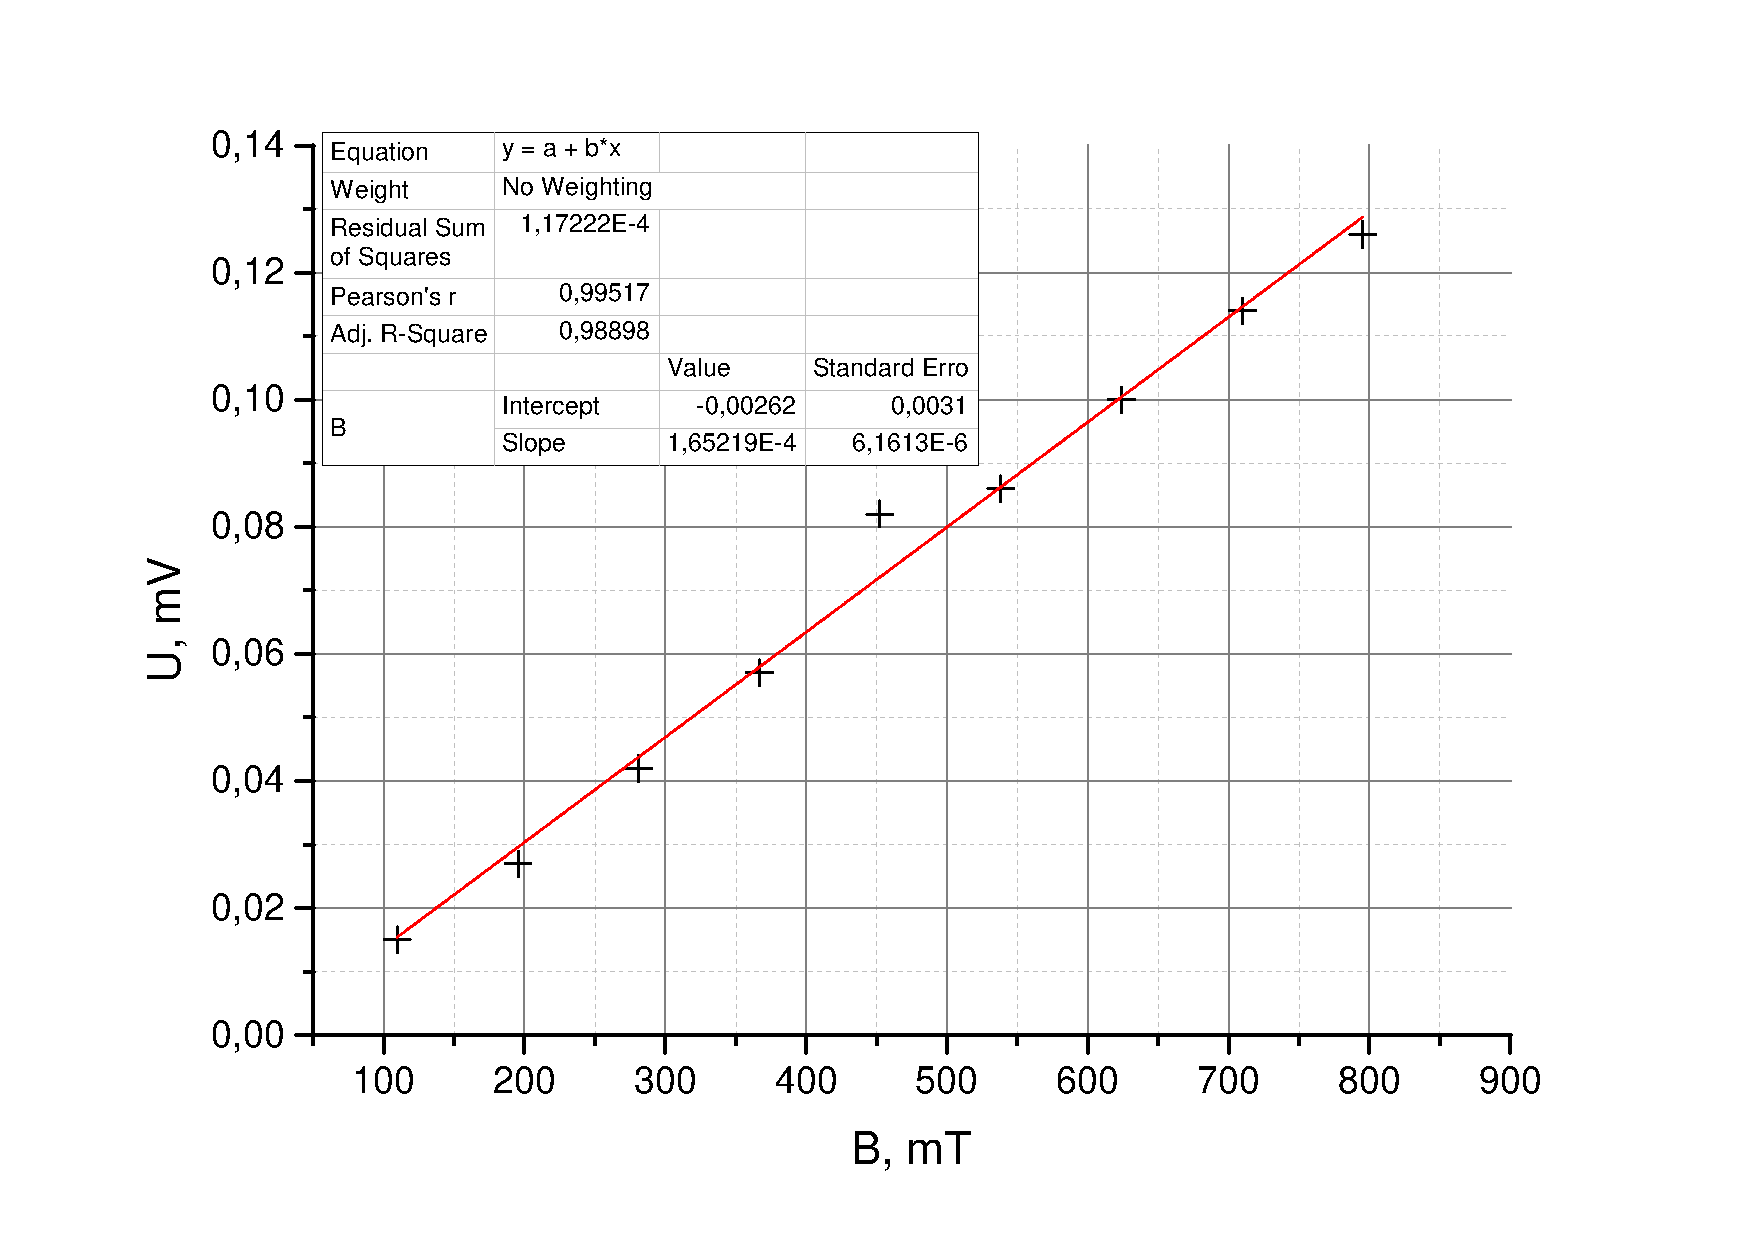
\includegraphics[width = 0.8\linewidth]{A04}
		
		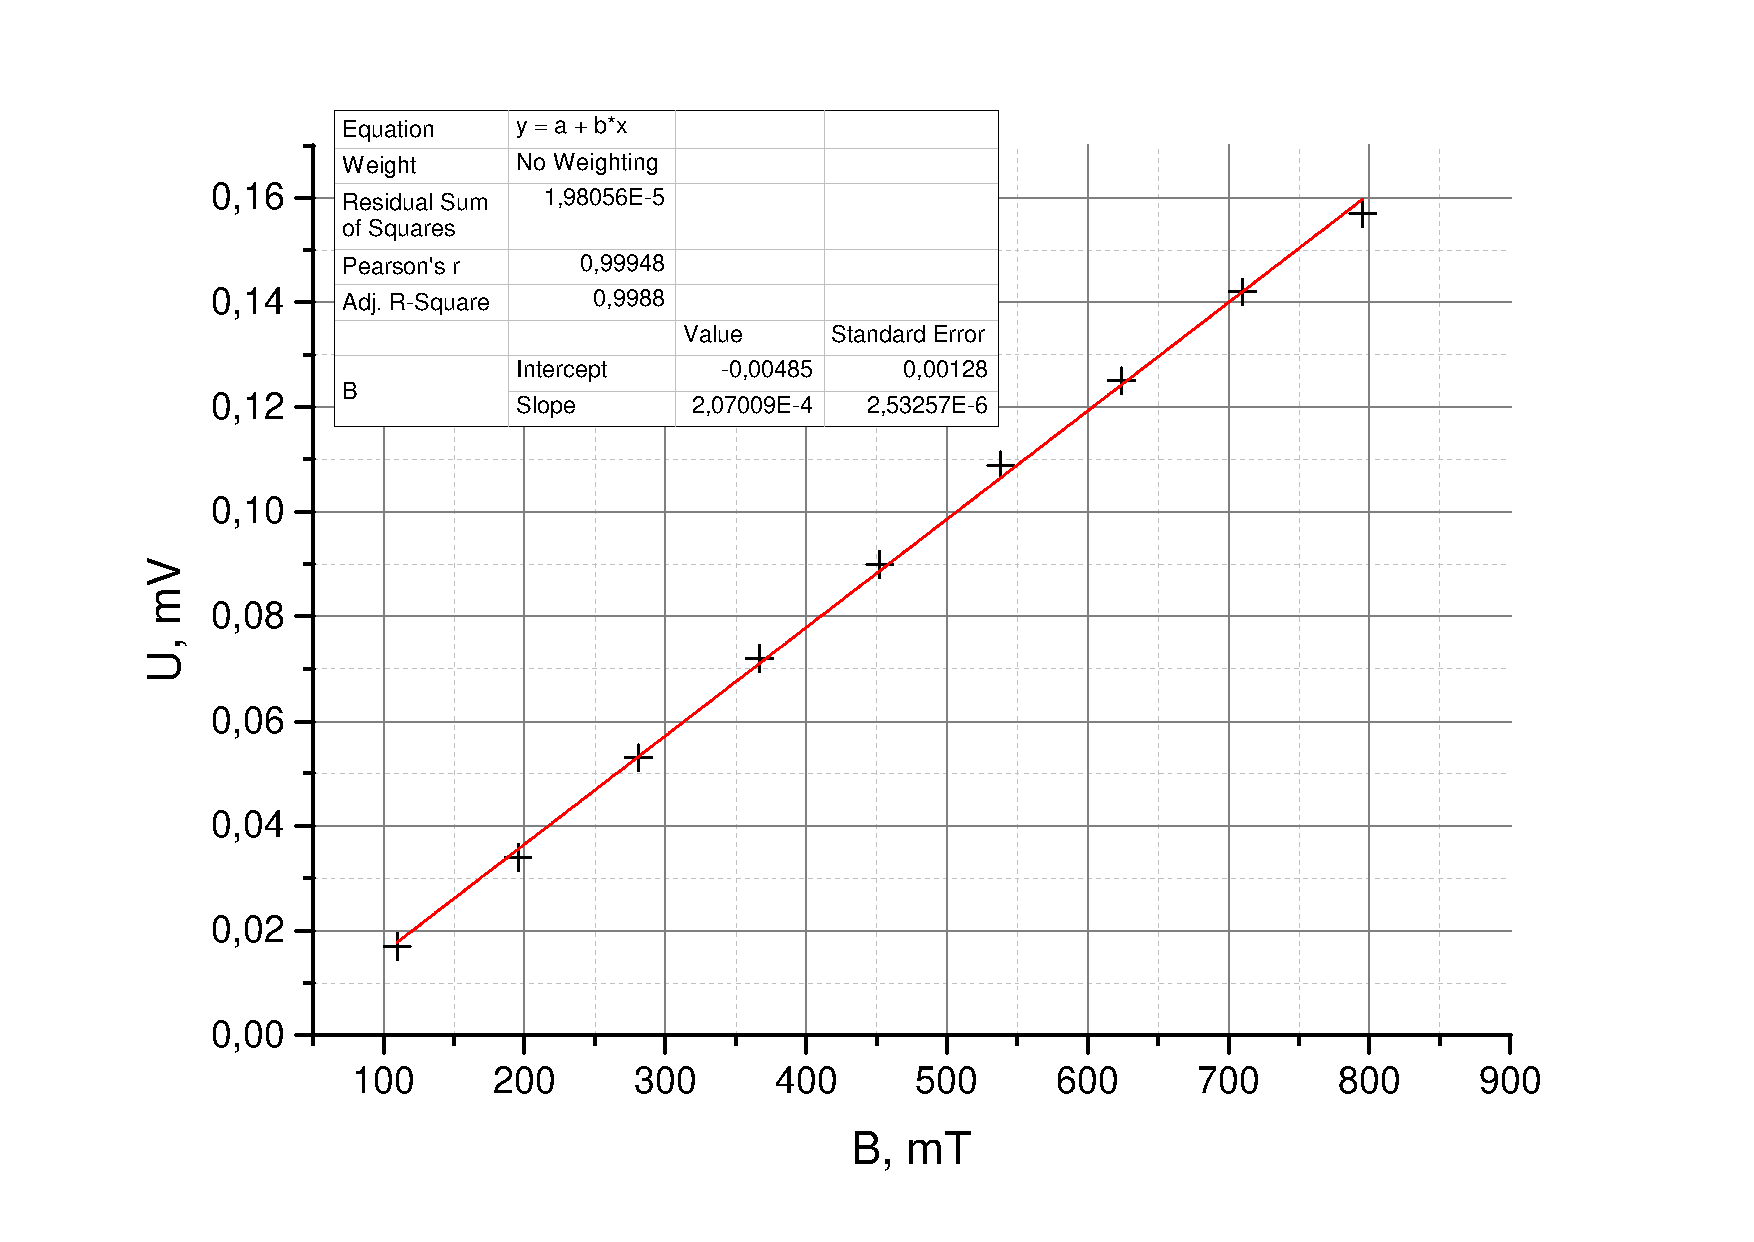
\includegraphics[width = 0.8\linewidth]{A05}
		
		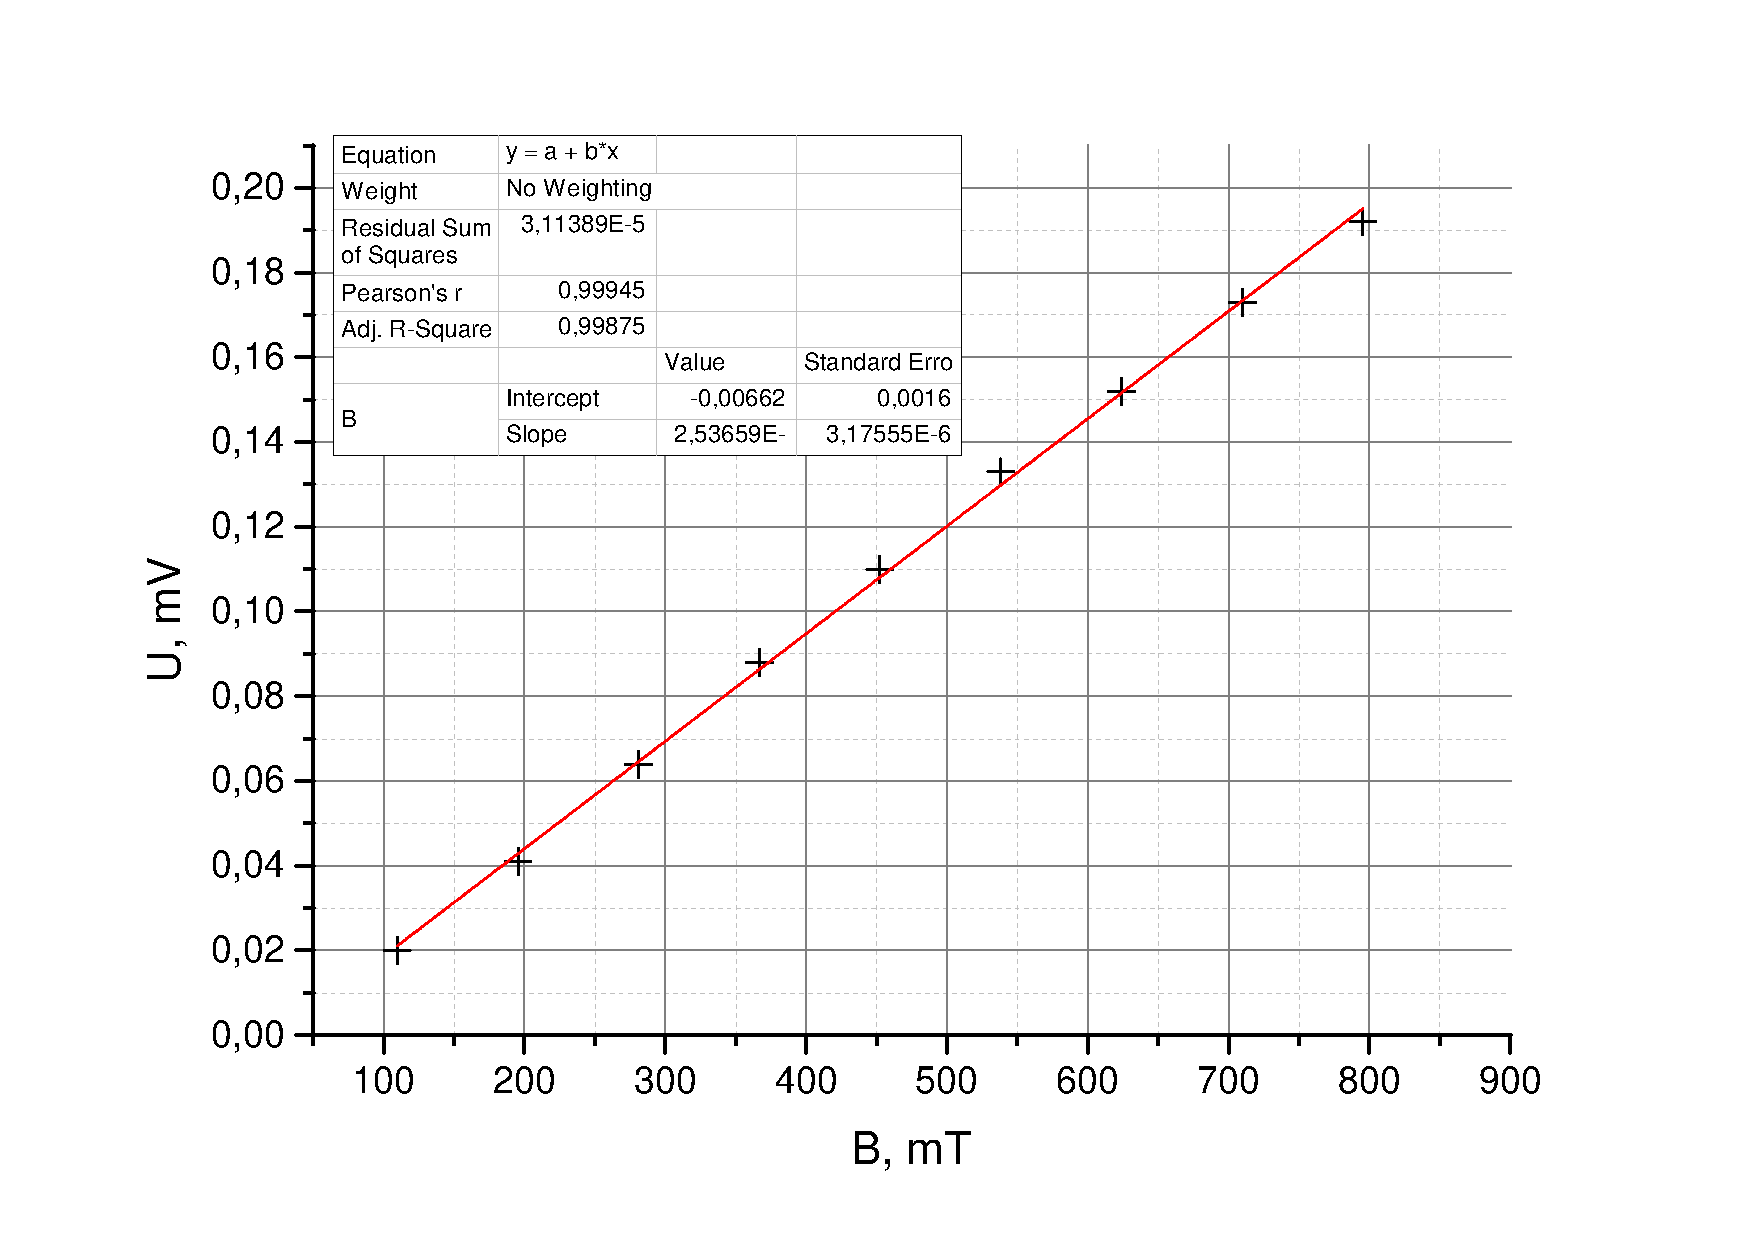
\includegraphics[width = 0.8\linewidth]{A06}
		
		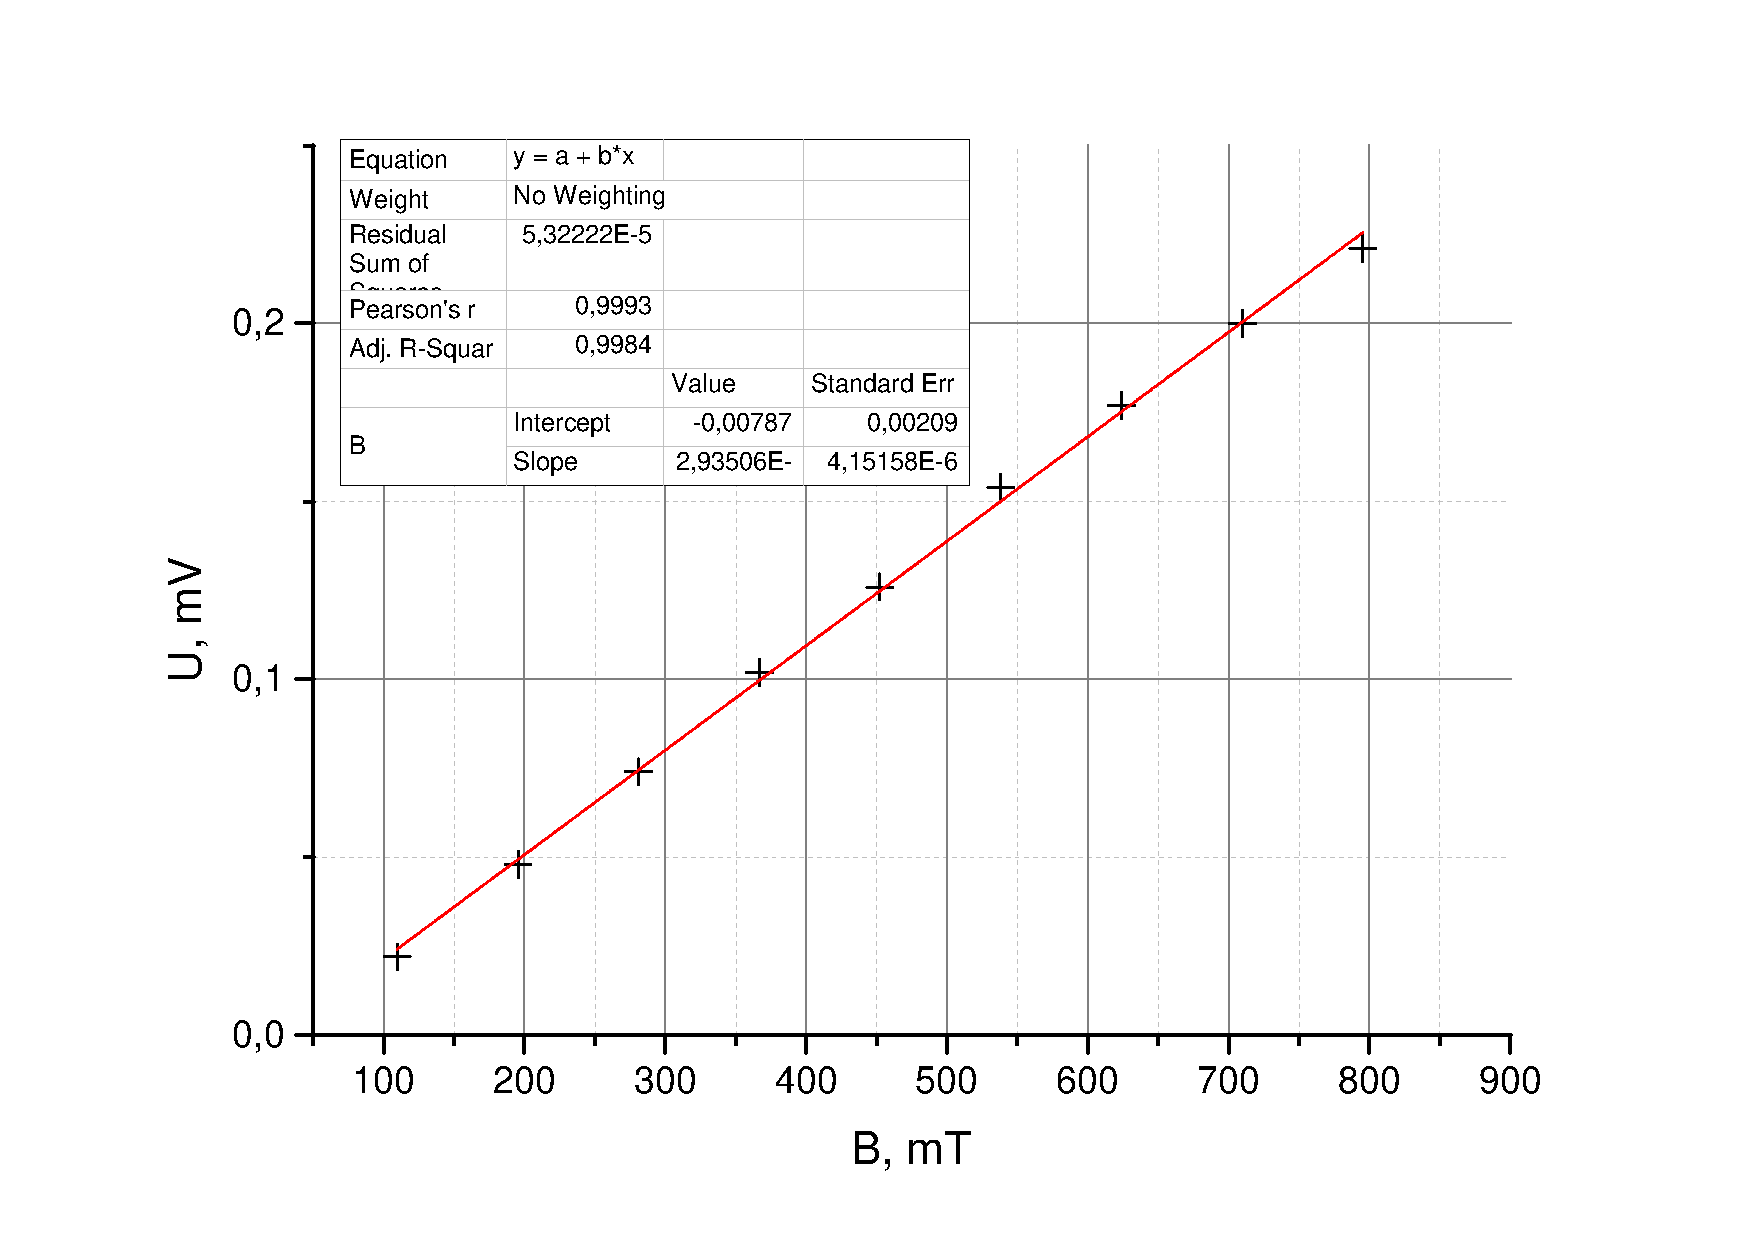
\includegraphics[width = 0.8\linewidth]{A07}
		
		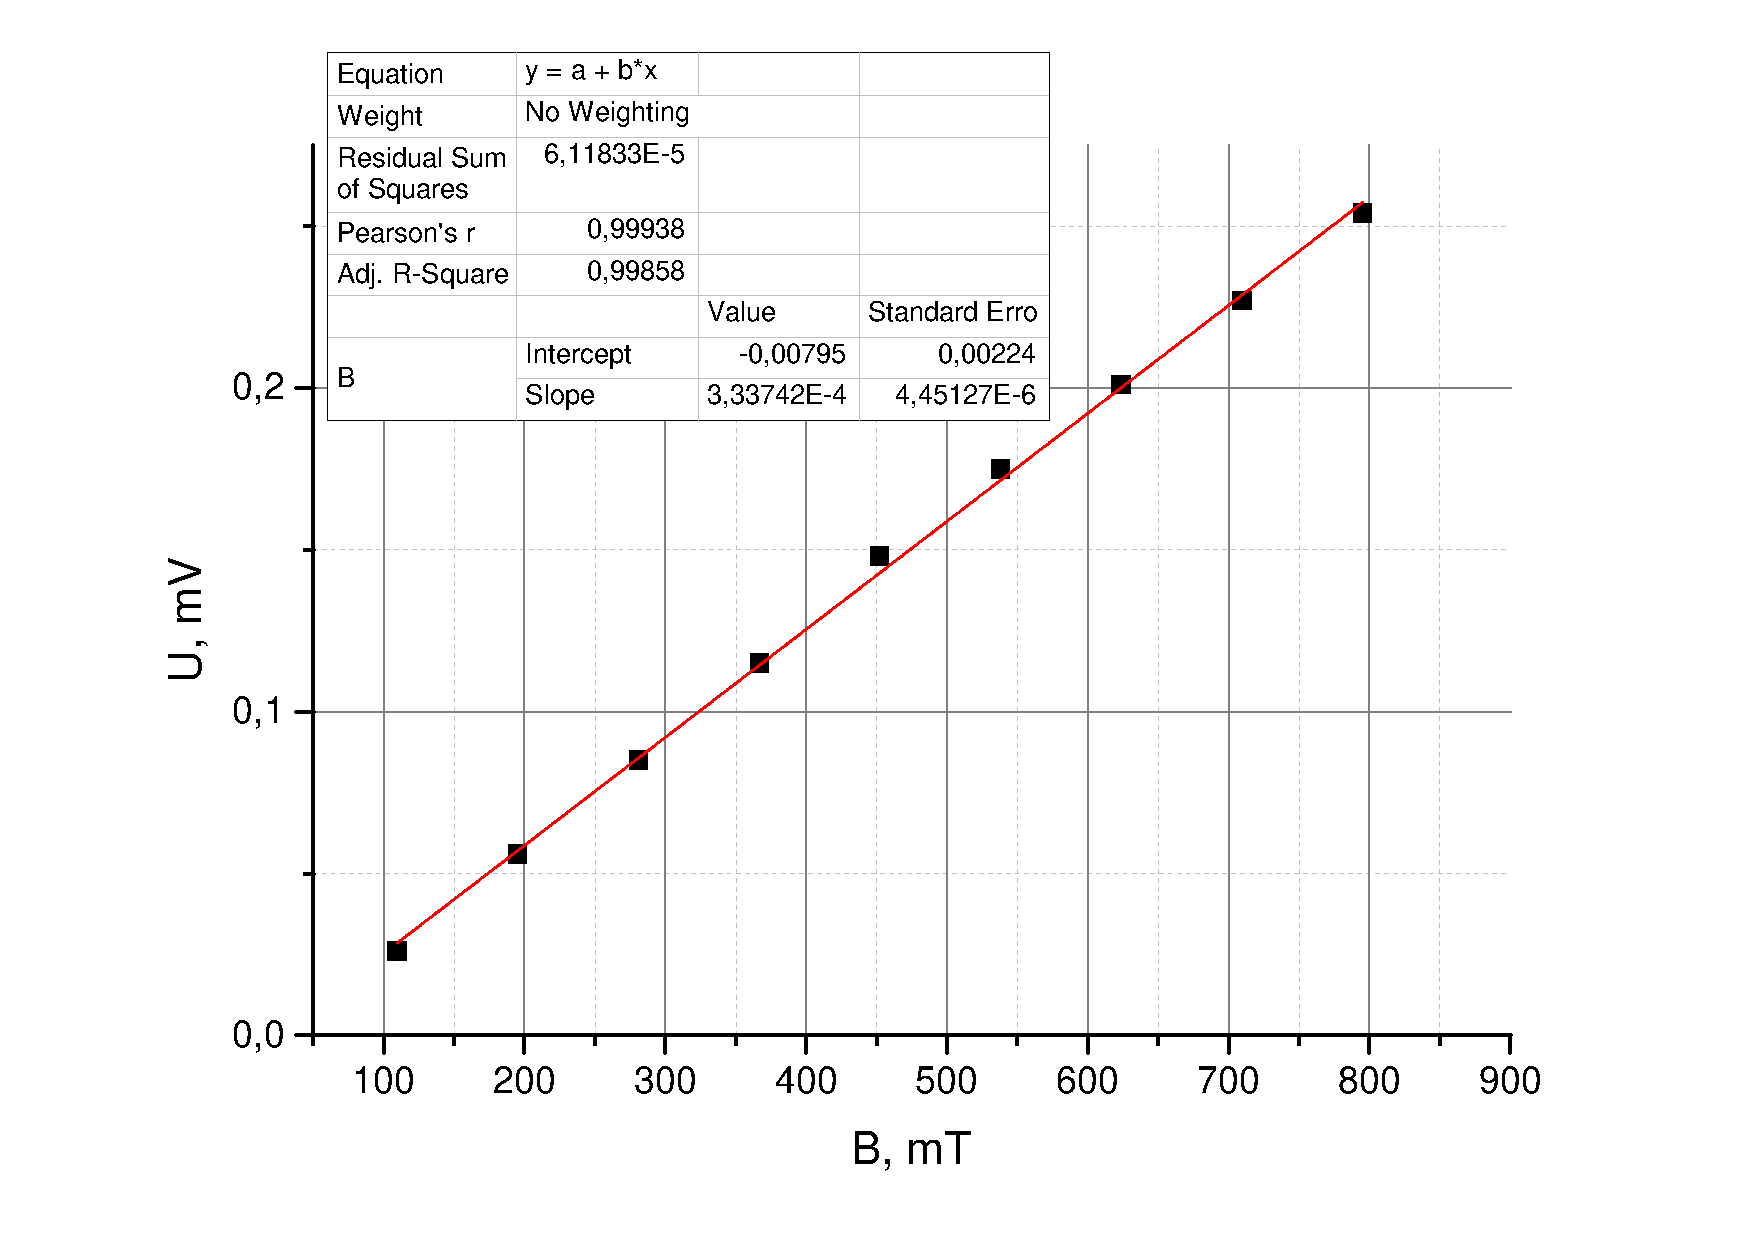
\includegraphics[width = 0.8\linewidth]{A08}
		
		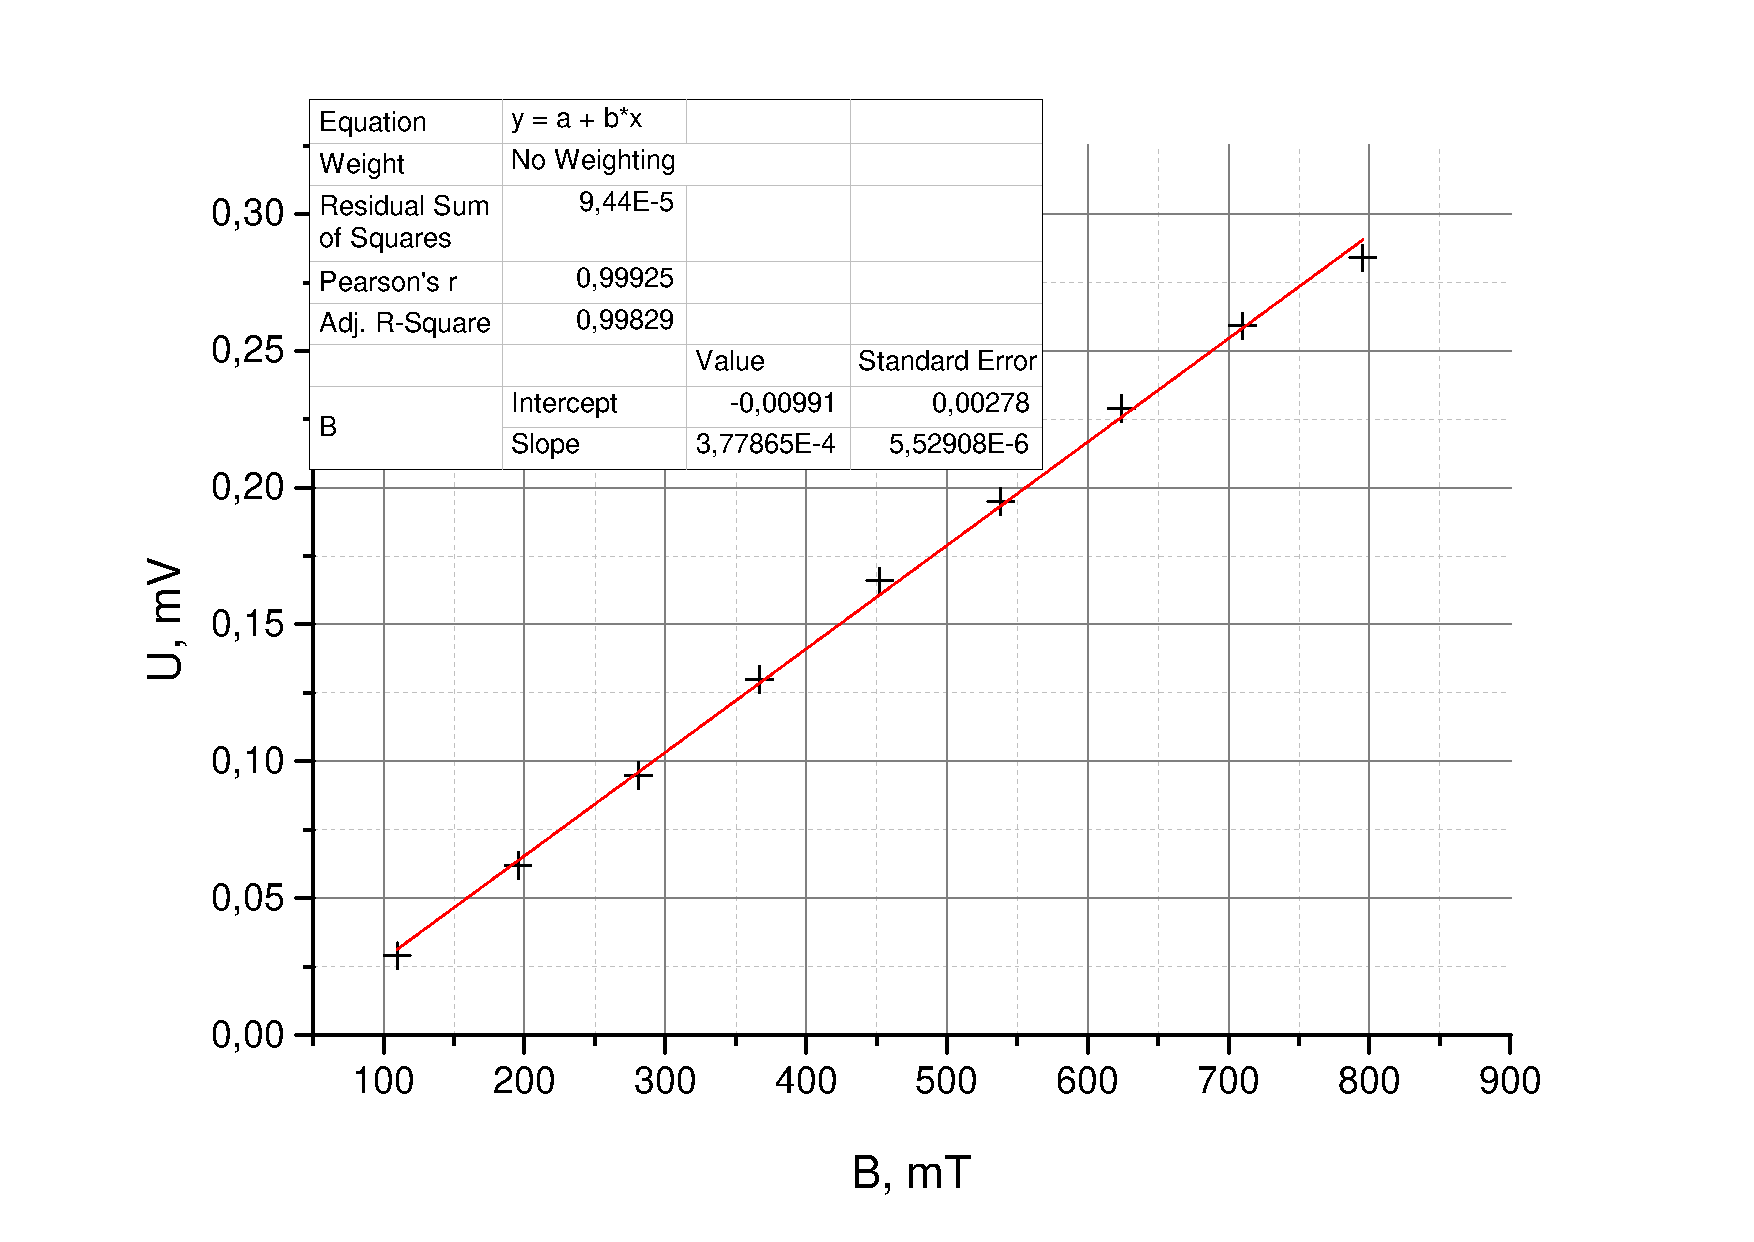
\includegraphics[width = 0.78\linewidth]{A09}
		
		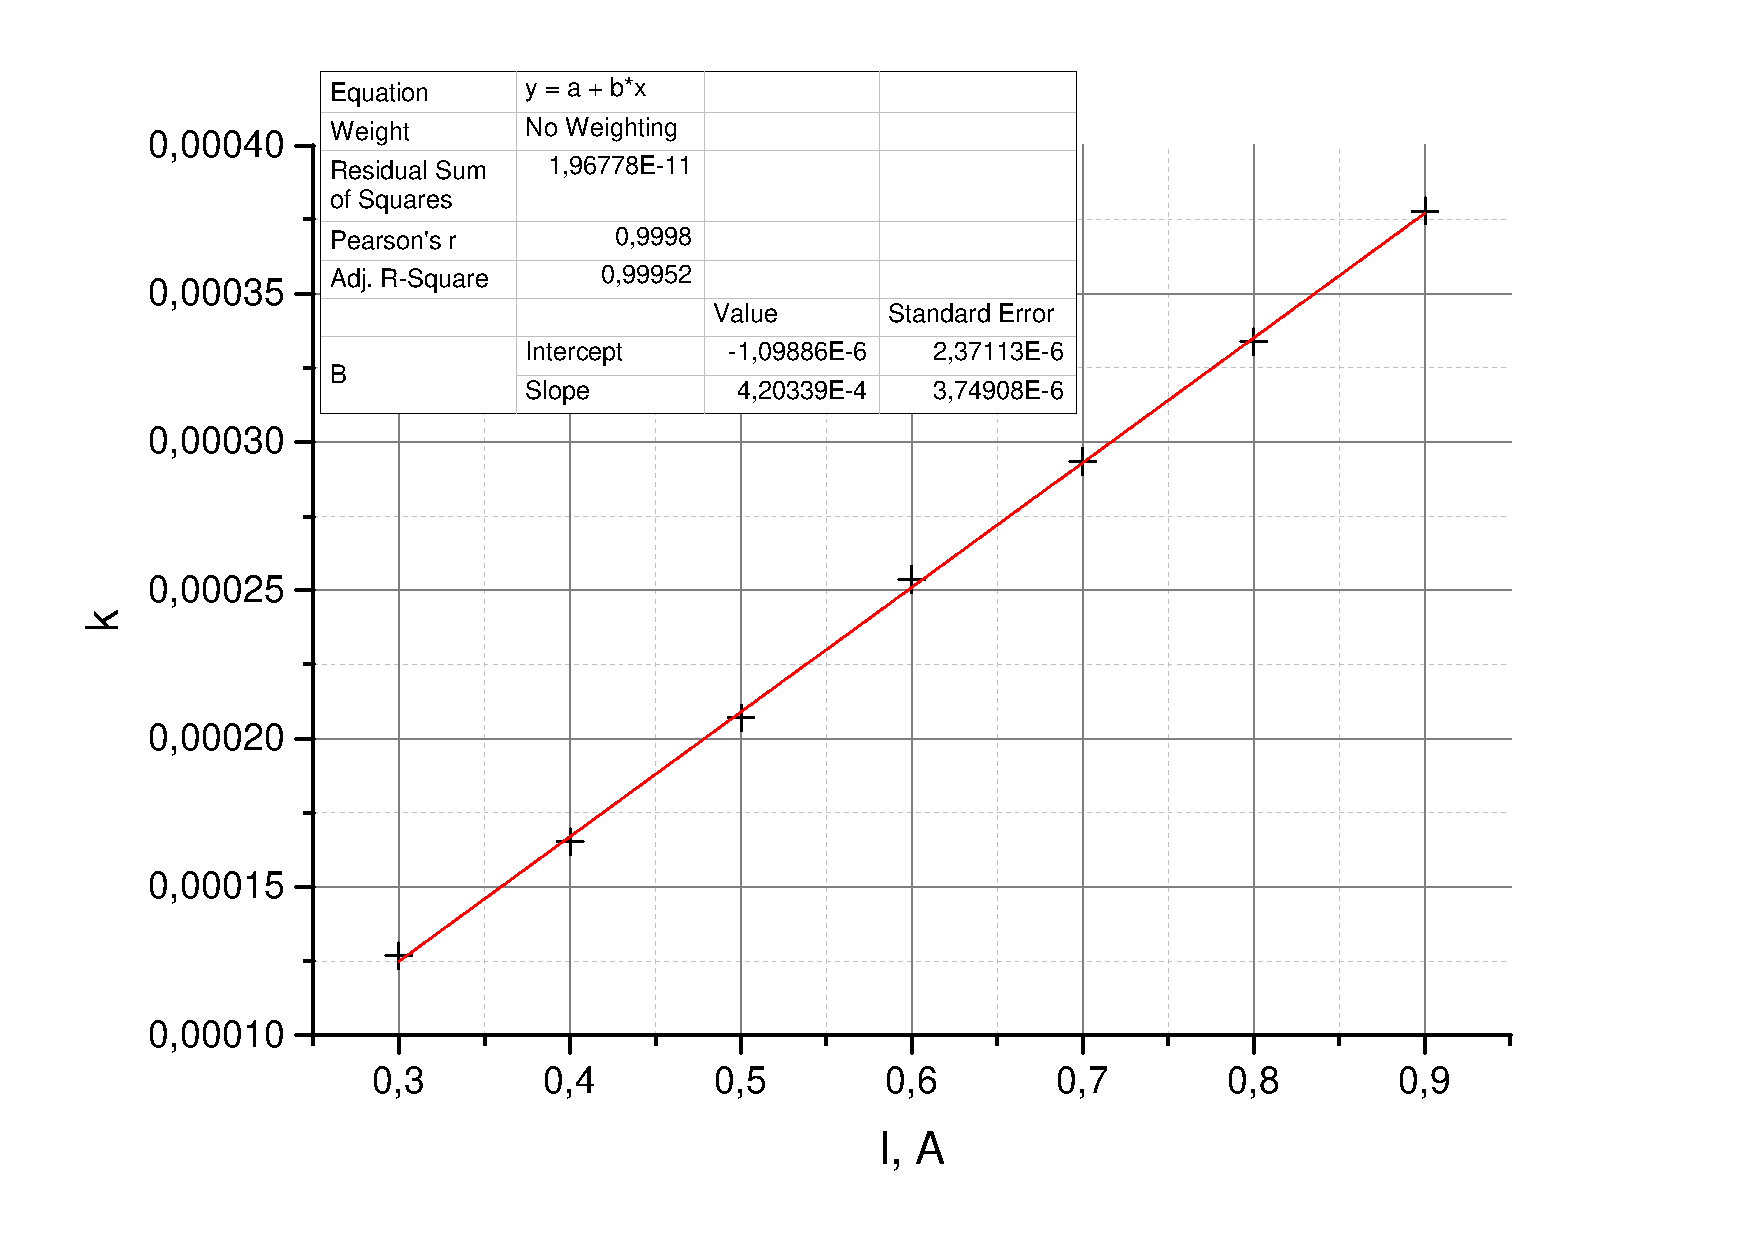
\includegraphics[width = 0.78\linewidth]{KFI}
		
		Рассчитаем константу Холла:
		\begin{equation}
			\upvarepsilon_x = -R_x\frac{IB}{a} \implies R_x = -ka = -4.2\cdot 10^{-4}\cdot 1.5\cdot 10^{-3} = \left(63 \pm 0.56\right)\cdot 10^{-6} \text{В}
		\end{equation}
		\begin{equation}
			\sigma = \frac{IL_{35}}{U_{35}al} = \frac{0.003}{1.673\cdot 0.0015\cdot 0.0017} = 703.21 \pm 14.06\, \frac{1}{\text{Ом}\cdot\text{м}}
		\end{equation}
		\begin{equation}
			b = \sigma R_x = 443.02\pm 9.69 \, \frac{\text{см}^2}{\text{В}\cdot\text{с}}
		\end{equation}
	\section{Вывод}
		К сожалению, в измерениях что-то пошло не так, и с табличными данными ничего не сошлось. Но в принципе, в полупроводниках можно наблюдать эффект Холла. Этот эффект применим в датчиках магнитного поля.
		
\end{document}


